\chapter{Pensamento Computacional}\label{pensamento-computacional}

\section{Computadores e as transformações na prática científica}
% A evolução da computação nos últimos anos, aliado ao seu barateamento, tem tornado possível o desenvolvimento de novas estratégias para resolução de problemas. Fato que tem produzido impactos notáveis tanto na academia quanto nas empresas.

% barateamento de capacidades computacionais de armazenamento e processamento

% As últimas 2 ou 3 décadas dominado - e o mundo transformado - pelo advento de computação cada vez mais poderosa, menos dispendiosa e onipresente, além do surgimento da World Wide Web e tecnologias relacionadas.


A evolução da computação nas últimas décadas, aliada ao seu barateamento, tem produzido impactos notáveis tanto na academia quanto na industria. A disponibilidade de dispositivos mais baratos e com maior capacidade de processamento e armazenamento tem tornado a computação ubiqua. 

% **Enriquecimento das formas de exploração de fenômenos.**

Na academia, esse fenômeno tem favorecido o surgimento de novas estratégias para exploração de fenômenos. Até meados do século 20, todo progresso cientifico foi conduzido apenas por interações entre atividades experimentais e analíticas\footnote{
Em sentido mais amplo, quando mencionamos `atividade analítica' estamos nos referindo à utilização de aparato matemático para resolução teórica de problemas. Ao mesmo tempo, o termo análise também pode fazer referência ao emprego da análise matemática, ramo da matemática que lida com conceitos do cálculo diferencial, tais como diferenciação, integração, e séries infinitas.}. O surgimento da computação e o seu desenvolvimento desde então trouxe consigo novas formas de fazer ciência, tais como a simulação e a modelagem computacional, e mais recentemente, a mineração de dados e o aprendizado de máquina, úteis para a análise de grande volume de informação \cite{Djorgovski2005, wing2006}. %TODO (cite weintrop, and wing)


O uso de simulações numéricas, por exemplo, se justifica ao permitir que um grande número de fenômenos muito complexos sejam analiticamente tratáveis. Em muitos casos essa é única forma de exploração possível. Mesmo na mecânica newtoniana mais simples, é possível resolver  exatamente, apenas, o problema de dois corpos. Para $N\geq3$, soluções numéricas são necessárias. Da astronomia podemos retirar alguns exemplos, como a formação de estrelas e galáxias e explosão estrelares - de modo geral, qualquer evento envolvendo turbulência  \cite[]{Djorgovski2005}. %weintrop

O uso de métodos computacionais, tal como a simulação, tem expandido a abrangência de sistemas não lineares que tem sido explorados pelo modelos matemáticos e computacionais. Como lembra \citeonline{Weintrop2016}, campos da ciência estão experimentando um renascimento de abordagens experimentais em razão do acesso facilitado a mais poder computacional. 

O autor destaca que num passado recente, para muitos pesquisadores apenas o estudo de sistemas determinísticos era viável, tendo o termo `não-linear', praticamente, o sinônimo de `insolúvel'. Havia desse modo a propensão à investigação computacional apenas de sistemas lineares. Esse quadro era especialmente verdade para muitas pesquisas em biologia e química. 

Esse processo ganha especial relevância ao nos darmos conta da natureza caótica da ampla maioria dos fenômenos físicos. Sistemas lineares e determinísticos são portanto exceções, e não a regra \cite[]{Weintrop2016}.

Outros agentes de transformações da prática científica, embora mais recentes e em fase nascente, são as novas possibilidades trazidas pela abundância e pelo barateamento do armazenamento grandes volumes de dados. Vivemos uma era onde a disponibilidade de dados gerados por câmeras, sensores, execução de simulações e registro de interação humana crescem exponencialmente. 

Nesse cenário, como ressalta \citeonline[]{Djorgovski2005}, o foco de valores tem mudado da propriedade de dados ou de instrumentos para reuni-los para a propriedade de conhecimento e ideas que tornam possíveis a extração de significados desse volume de informação. 

A abundância traz consigo muitos desafios. A taxa com que cientistas e engenheiros têm coletado e produzido dados vem exigindo avanços nas estratégias de análise. O acúmulo chegou a um nível de complexidade que, certo modo, tem sido impossível fazer qualquer tipo de investigação superficial utilizando técnicas convencionais, baseadas na percepção humana. Lidar com esse conjunto desestruturado e rico de dados, extraindo dele significado, tem sido uma das batalhas da atual revolução científica e industrial \cite[]{Djorgovski2005}. Nesse contexto o emprego de técnicas de aprendizado de máquina é essencial.

Em linhas gerais, o aprendizado de máquina (do inglês: \textit{machine learning}) basea-se no uso algoritmos que instruem computadores sobre como avaliar dados e deles extrair padrões e correlações, permitindo-os, de forma extraordinária, a fazer predições. E esse processo tem um componente recursivo: quanto mais análises são feitas, mais experiência e competência são adquiridas. Ou seja, mais `inteligentes' essas máquinas se tornam.

\citeonline[]{Escobar} propõe uma visão simplificada das interações humanas que facilita o entendimento desses algoritmos. Como descreve, ao conhecemos alguém pela primeira vez, baseando-nos em modelos pessoais, somos capazes de dizer nos primeiros minutos se essa pessoa nos transmite boa ou má impressão. Para cada nova pessoa que encontramos, avaliamos algumas de suas características e as registramos. Esse processo nos permite refinar e recompor modelos sociais que irão influenciar outras percepções em interações futuras. 

É exatamente nesse princípio recursivo que se fundamenta o aprendizado de máquina: categorizar dados de acordo com suas características com o fim de compor e refinar modelos.

Esse processo tem se provado extremamente eficiente na predição da configuração de sistemas estocásticos. Tomemos por exemplo a necessidade de prever o tempo, onde há dominância de comportamentos turbulentos. Em um estudo recente \apud[]{PhysRevLett.120.024102}{Vutha}, mostrou-se a eficiência do uso de algoritmos de inteligência artificial para previsões ao longo de um período muito maior do que se imaginou possível. Um ponto digno de nota: o algoritmo utilizado não continha nenhuma informação sobre as equações subjacentes. 

Há atualmente questionamentos sobre até que ponto o uso intensivo de `robôs oráculos' levará à perda pelo interesse dos pesquisadores em descrever fenômenos em termos de equações e princípios unificadores. Esse debate é sintetizado pela confronto das noções de ``predição'' e ``entendimento''.

\citeonline[]{Vutha} expõe os elementos desse debate com um exemplo histórico. Como destaca, durante mais de um milênio, o movimento dos planetas eram descritos a partir de um modelo elaborado por Ptolomeu, cujos métodos lançavam mão de cálculos misteriosos envolvendo sobreposição de círculos. Apesar de ignorar a teoria da gravidade e de ter a Terra no centro do Universo, esse modelo foi extremamente eficiente na sua capacidade preditiva. Contudo, ele não oferecia nenhum entendimento capaz de explicar o seu funcionamento.

\begin{figure}[htb]
	\caption{\label{Ptolomeu} Modelo geocêntrico de Ptolomeu}
	\begin{center}
	    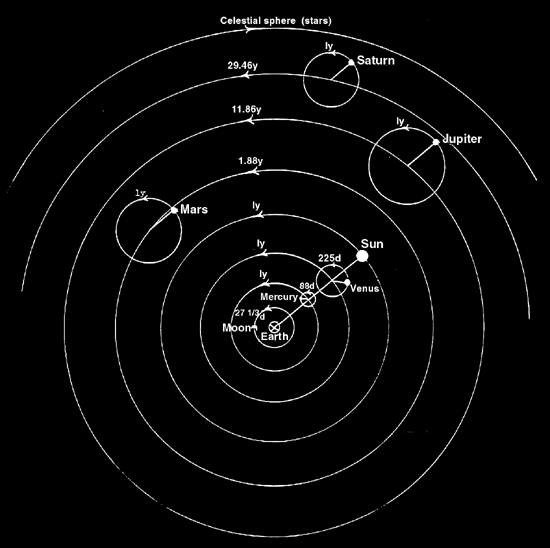
\includegraphics[scale=0.5]{imagens/ptolemy}
	\end{center}
	\legend{Fonte: \citeonline[]{Hatch}}
\end{figure}

A descrição do movimento dos corpos celestes só foi finalmente compreendida a partir da equações diferenciais descobertas por Isaac Newton. Com elas tem sido possível, desde então, prever a trajetória de todo e qualquer planeta do sistema solar.

A qualidade da proposta de Newton estava na possibilidade de oferecer não apenas a descrição de trajetórias, mas por permitir também que entendamos o porquê que elas são de uma e não de outra forma. Ao nos trazer equações, ele nos facultou a compreensão do fenômeno do movimento a partir da ótica de princípios unificadores. E é exatamente nesse ponto que reside o poder da descrição matemática. Como analisa \citeonline{Vutha}, se formos capazes de extrair de um fenômeno complicado dois ou três princípios, podemos dizer então que o compreendemos.

Porém, dada a dominância de fenômenos complexos na natureza, tem sido extremamente difícil extrair de muitos deles princípios simples. Descrevê-los, portanto, a partir da obtenção de equações universalmente válidas pode ser uma forma um tanto ineficiente de gerar predições relevantes \cite{Vutha}. O emprego de técnicas de \textit{machine learning}, nesse sentido, tem sido essencial.

A inteligência artificial tem ocupados outros espaços além da pesquisa científica. Desde robôs que leem a web para tomar decisão de investimentos \cite[]{Bloomberg} e carros que se auto dirigem, até contextos relativamente mais simples como tradutores automáticos e mecanismo buscas. Já no mundo do trabalho, um sem-número de projeções apontam para a substituição progressiva de quantidade considerável de atividades laborais por robôs.


\begin{figure}[htb]
	\begin{center}
	    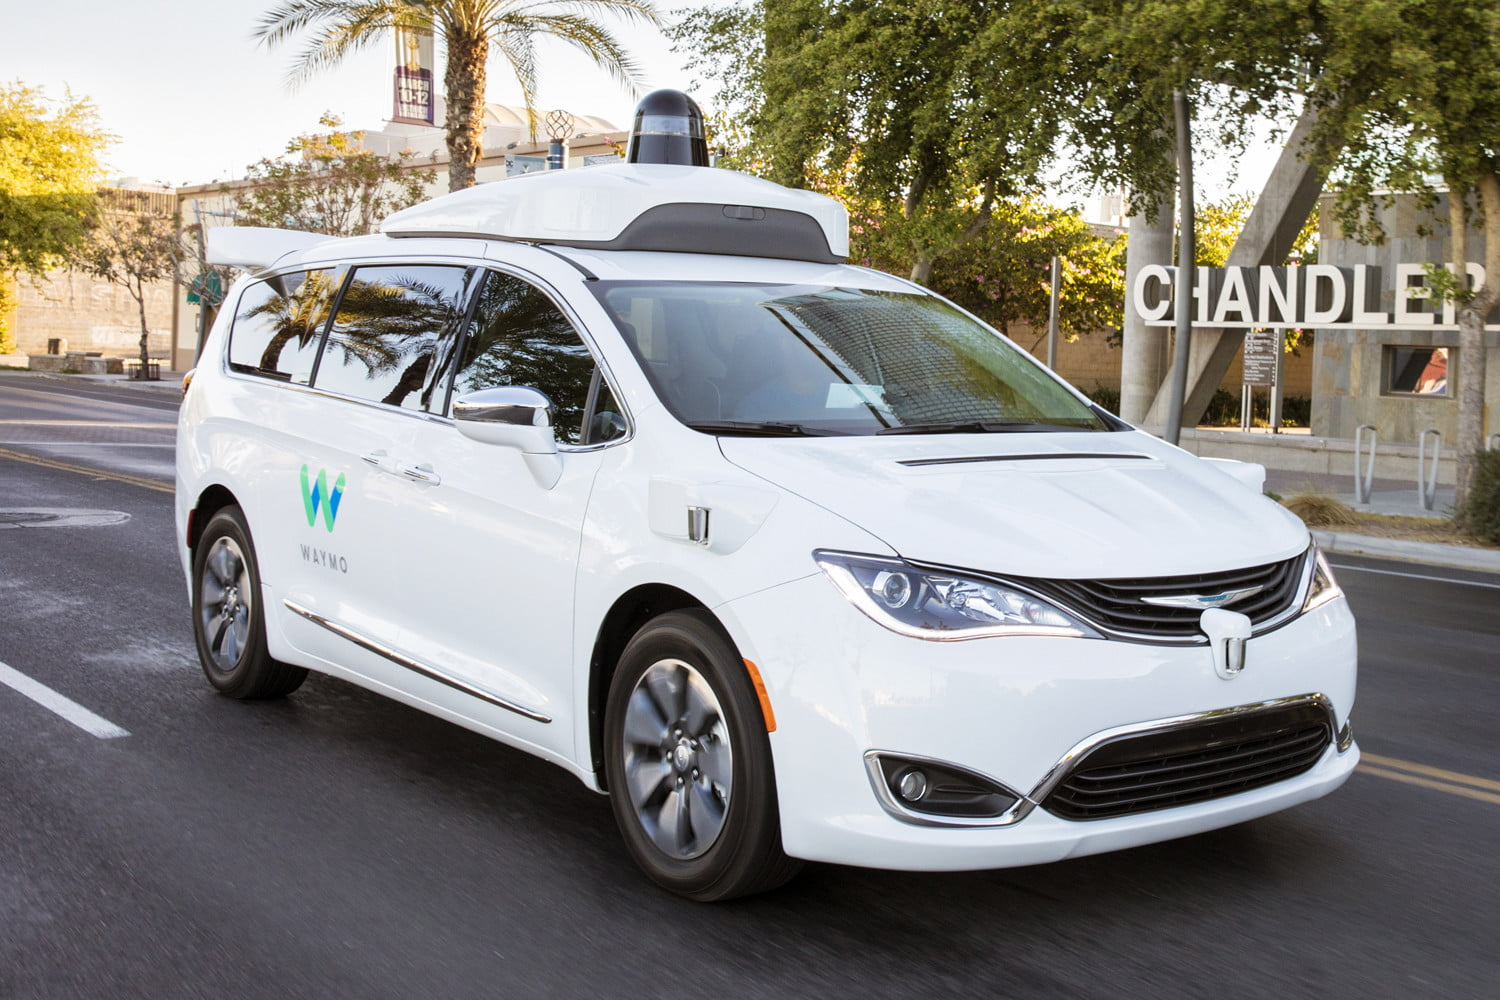
\includegraphics[scale=0.25]{imagens/waymo}
	\end{center}
	\caption{\label{Waymo} Carro autônomo da Waymo, subsidiária de veículos da Alphabet (matriz do Google)}
\end{figure}

A produção estratosférica de dados e a invasão da inteligência artificial nos meios científicos e na indústria é sintomático da interação dinâmica entre a ciência, a tecnologia, e a sociedade em ciclos que se retroalimentam.

Novas descobertas levam a novas perguntas que exigem mais coleta de dados. Quando analisadas, essas informações são utilizadas para refinar e ajustar modelos, levando a novas perguntas e mais produção de dados. Esse processo tende a culminar na criação de novas tecnologias. Tecnologias, por seu turno, inspiram usos sociais criativos que quase sempre criam demandas por mais descobertas científicas e mais tecnologia. Sob esse aspecto, podemos dizer que esses três atores desempenham o papel de forças motrizes da computação \cite[]{wing2008}. 

\begin{figure}[htb]
	\caption{Forças motrizes da computação}
	\begin{center}
	    
\includegraphics[scale=0.28]{imagens/forcas_motriz.png}
	\end{center}
	\legend{Adaptado de \citeonline[]{wing2008}}
\end{figure}

O barateamento dos custos de produção científica é outro aspecto relevante dessas transformações. À medida que a internet e dados, consequentemente, se tornam mais acessíveis, qualquer pessoa com boas ideias e bons hábitos de trabalho, de qualquer lugar, pode fazer ciência de primeira linha, comunicar seus resultados e aprender com a comunidade científica. Essa possibilidade é especialmente benéfica para países e instituições que não dispõem de instalações sofisticadas \cite[]{Djorgovski2005}. 

Sobre o papel da ciência da computação no desenvolvimento científico, \citeonline[]{Djorgovski2005} faz um consideração provocativa: 

\begin{citacao}
	$[...]$ a ciência da computação aplicada está desempenhando o papel que a matemática fez do século XVII ao século XX: fornecer uma estrutura ordenada e formal e um aparato exploratório para outras ciências. Além de seu aparentemente feliz caso com a teoria das cordas, é difícil dizer o que a matemática está fazendo para outras ciências hoje. A maioria dos cientistas de matemática que utilizamos hoje foi desenvolvida há mais de um século. \cite[p.~131. Tradução nossa]{Djorgovski2005}
\end{citacao}

E é do do seio dessa reflexão que nasce a noção de um ``pensamento computacional''. Tema que desdobraremos a seguir.

\vspace{1cm}

\section{A consolidação da ciência da computação na investigação científica: o pensamento computacional}

A noção de pensamento computacional tem ganhado força desde 2006, ano em que a professora Jeannette Wing, então professora da Universidade Carnegie Mellon, publica um artigo seminal no qual propõe um conjunto de atitudes, ou abordagens, para a resolução de problemas fundamentadas na forma como cientistas da computação e programadores tratam problemas computacionais. 

A definição clássica que muitos autores dão para o conceito é extraído do próprio trabalho da autora. Como segue, o pensamento computacional consiste ``numa abordagem para a solução de problemas, desenho de sistemas e entendimento do comportamento humano que se vale de conceitos fundamentais para ciência da computação'' \cite[Tradução nossa]{wing2006}.

Um dos pilares que sustenta sua proposta é o conceito de abstração. Nas suas palavras, 

Um dos elementos que ganha centralidade na sua proposta é a noção de abstração. 


% O emprego dessa expressão contudo não é nova.



% Aprendizado de máquina, ou simplesmente inteligência artificial, basea-se grosso modo 

% Outra idéia levemente provocativa é que a ciência da computação aplicada está desempenhando o papel que a matemática fez do século XVII ao século XX: fornecer uma estrutura ordenada e formal e um aparato exploratório para outras ciências. Além de seu aparentemente feliz caso com a teoria das cordas, é difícil dizer o que a matemática está fazendo para outras ciências hoje; A maioria dos cientistas de matemática que utilizamos hoje foi desenvolvida há mais de um século.

% Recente avanços na computação de alta velocidade e em metdos analiticos criou ferramentas poderas para entender fenomenos em todos os espectros do pensamento humano (human inquiry)

%Wing(2006) argumenta que o pensamento computacional se tornaria fundamental pra todas as disicplinas que os avanços na computação habilitaria pesquisadores para desenvolver (envision) novas estrategias de resolução de problemas e teste de novas soluções.

%Todo o desenvolvimento científico até meados do século 20 se deu a partir do uso atividades analiticas e experimentais.

%**Simulação e modelagem computacional**

